\begin{document}
%%%% Liikennesuunnitelmat

\hrule $\color{white}{.}$ \\
Merkitään 
\begin{itemize}
    \item $\mathcal{B}$ Borelin $\sigma$-algebra joukossa $K$
    \item $\Omega = [0,|\Omega|]$, kaikkien säikeiden indeksijoukko. (Kirjan johdannossa valittu [0,1])
    \item $X$ kompakti, konveksi $R^n$ osajoukko, $X \subset R^n$.
    \item $|A|$ Mitallisen joukon $A\subset \R$ Lebesgue-mitta.
    \item $K$ Merkitään kaikkien 1-Lipschitz kuvauksien $\gamma:\R^+ \to X$ joukkoa $K$. 
    \item $\mathcal{P}(E)$ joukon $E$ osajoukkojen kokoelmaa
\end{itemize}
\hrule


\begin{definition}
    Määritellään etäisyys joukossa $K$ siten, että
    \[d(\gamma, \gamma') = \sup_k \frac{1}{k}||\gamma - \gamma||_{L^\infty([0,k])}\]
\end{definition}

\begin{definition}
    Määritellään polun $\gamma \in K$ pysähtymisajaksi 
    \begin{equation*}
        T(\gamma) = \inf\{t\ge0:\gamma \text{ vakio välillä } [t,\infty[ \}
    \end{equation*}
    ja pituudeksi $L(\gamma)$ polun pituus välillä $[0, T(\gamma)]$ eli
     \begin{equation*}
         L(\gamma) = \int_0^{T(\gamma)}|\gamma'(t)|\, \dt.
     \end{equation*}
\end{definition}

Pysähtymisajalla kuvastetaan luonnollisesti sitä, mistä parametrin arvosta $t$ lähtien polku $\gamma$ pysyy paikoillaan. 

\begin{definition}\label{def:liikennesuunnitelma}
    Mitta $\P: K \to \R^+$ avaruudessa  $(K, \Borel)$ on \textbf{liikennesuunnitelma}, jos
    \begin{equation*}
     \int_K T(\gamma) \, \d \P (\gamma) < \infty.   
    \end{equation*}
\end{definition}

\begin{definition}
    Olkoon $\P$ liikennesuunnitelma. Merkitään joukon $X$ kaikkia liikennesuunnitelmia $TP = TP(X)$, ja $TP_C = TP_C(X)$ kaikkia joukon $X$ liikennesuunitelmia $\P$ joille
    \begin{equation*}
        \int_K T(\gamma) \d \P(\gamma) \le C.
    \end{equation*}
\end{definition}

\begin{definition}
    Olkoon $\pi_0, \pi_\infty: K\to X$ ja $\pi:K\to X \times X$ kuvauksia, jotka määritellään polulle $\gamma \in K$ siten, että 
    \begin{align*}
        \pi_0(\gamma) &= \gamma(0) &&\Big| \text{ Polun lähtöpiste. }\\
        \pi_\infty(\gamma) &= \gamma(T(\gamma)) &&\Big| \text{ Polun päätepiste. }\\
        \pi(\gamma) &= (\gamma(0), \gamma(T(\gamma)) &&\Big| \text{ Polun lähtöpiste ja päätepiste. }
    \end{align*}
\end{definition}

\begin{definition}
    Määritellään mitat $\mu^+, \mu^- : X \to \mathbf{R}_+$ ja $\pi: X\times X \to \mathbf{R}_+$ siten, että
    \begin{align*}
        \mu^+(\P) &= \pi_{0\#} \P  &&\Big| \text{ Irrigoiva mitta, \textit{irrigating measure} }\\
        \mu^-(\P) &= \pi_{\infty \#} \P  &&\Big| \text{ Irrigoitu mitta, \textit{irrigating measure} }\\
        \pi(\P) &= \pi_\# \P  &&\Big| \text{ Siirtosuunnitelma liikennesuunnitelmalle $\P$,}\\ 
        & &&\hphantom{\Big|} \text{ \textit{transference plan of $\P$}}
    \end{align*}
\end{definition}

\begin{figure}
    \centering
    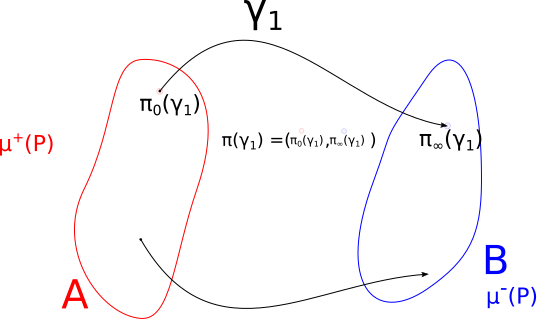
\includegraphics[scale=0.8]{graphics/irrigoiva-ja-irrigoitu-mitta.png}
    \caption{Havainnollistus sovituista merkinnöistä.}
    \label{fig:my_label}
\end{figure}


\begin{remark}
    Kaikille Borelin joukoille $A, B \subset K$ pätee
    \begin{align*}
        \mu^+(\P)(A) &= \P(\pi_0^{-1}(A)) = \P(\{\gamma \in K : \gamma(0) \in A\}) \\
        \mu^-(\P)(B) &= \P(\pi_\infty^{-1}(B)) = \P(\{\gamma \in K : \gamma(\infty) \in B\}) \\
        \pi(\P)(A\times B) &= \P(\pi(A\times B)) = \P(\{\gamma \in K: \gamma(0) \in A\text{ ja } \gamma(\infty) \in B)\}
    \end{align*}
\end{remark}

Liikennesuunnitelman irrigoiva mitta on mitta sille joukolle, mistä massaa ollaan lähettämässä ja irrigoitu mitta mihin sitä ollaan lähettämässä. Liikennesuunnitelman siirtosuunnitelma sisältää tiedon siitä minne mikäkin massa lähetetään.

\subsection{Parametrisoidut liikennesuunnitelmat}
 
\begin{theorem}
    Olkoon $\P: K \to \R^+$ liikennesuunnitelma. Tällöin on olemassa mitallinen funktio $\chi: [0, c] \to K$ siten, että liikennesuunnitelma voidaan kirjoittaa muodossa $$\P =\chi_\# \lambda.$$
\end{theorem}
\begin{proof}
    Lause seuraa Skorohkodin lauseesta.
\end{proof}
Skorohkodin lauseen mukaan mikä tahansa liikennesuunnitelma $\P$ voidaan parametrisoida mitallisella funktiolla $ \chi: [0, c] \to K$ s. e. $\P = \chi_\# \lambda$, missä $\lambda$ on Lebesguen mitta välille $[0,c]$. 

Funktio $ \chi:[0, c] \to K$ antaa siis jokaiselle välin $[0, c]$ luvulle 1-Lipschitz-polun joukosta $K$. 
Merkitään jatkossa $\Omega = [0,c]$ ja kutsutaan väliä indeksijoukoksi. Polku $ \chi(\omega)$ vastaa siis indeksin $\omega$ hiukkasen reittiä.

Merkitään nyt $\chi(\omega, t) :=  \chi(\omega)(t)$ kaikille $\omega \in \Omega$ ja $t \in \R^+$. Jatkossa, kun käytetään merkintää $\chi(\omega, t)$, tarkoitetaan siis funktiota $\chi : \Omega \times \R^+ \to X$. Osoitetaan seuraavaksi, että myös näin määriteltynä $\chi$ on mitallinen funktio.

\begin{theorem}
    Funktio $\chi: \Omega \times \R^+ \to X $ on mitallinen jos funktio $ \chi: \Omega \to K$ on mitallinen.
\end{theorem}
\begin{proof}
Bernot, Caselles: Optimal transportation networks s.27 (joss.-versio)
\end{proof}
Funktion $\chi$ pysähdysaika määritellään vastaavasti, kuten liikennesuunnitelman $\P$ pysähdysaika.
\begin{definition}
    Jos $\chi: \Omega \times \R^+ \to X$ on mitallinen, niin sen \textit{pysähdysaika} $T_\chi$ on
    \[T_\chi (\omega) = \inf\{t : \chi(\omega, t) \text{ on vakio välillä } [t,\infty[\}\]
\end{definition}

\begin{definition}
    Olkoon $\Omega \subset \R$ Lebesgue-mitallinen ja Lebesgue-mitaltaan äärellismittainen. Mitallinen kuvaus $\chi: \Omega \times \R^+ \to X$ on \textbf{parametrisoitu liikennesuunnitelma}, jos $t\to \chi(w,t)$ on 1-Lipschitz kaikille $\omega \in \Omega$ ja
    \[\int_\Omega T_\chi (\omega) \, \d \omega < \infty .\]
\end{definition}

\begin{definition}
    Olkoon $\Omega\subset \R$ mitallinen ja äärellismittainen. 
    \begin{itemize}
        \item Funktio $\chi:\Omega \times \R^+ \to X$ on tällöin \textit{parametrisoitu liikennesuunnitelma}. \item Polkua $\chi(\omega, \cdot)$ kutsutaan \textit{säikeeksi}.
        \item Polun $\chi(\omega, \cdot)$ kuvajoukkoa kutsutaan myös \textit{säikeeksi}.
    \end{itemize}
\end{definition}

\begin{theorem}\label{thm:push-cov}
    Olkoon Borelin avaruudet $(X_1, \Sigma_1)$ ja $(X_2, \Sigma_2)$, mitallinen kuvaus $f: X_1 \to X_2$ ja mitta $\mu:\Sigma_1 \to [0, \infty]$. \what{Mikä on g?} Tällöin
    
    \begin{equation*}
        \int_{X_2} g \, d(f_{\#} \mu) = \int_{X_1} g \circ f \, d\mu.
    \end{equation*}
\end{theorem}
\begin{proof}
LÄHDE?
\end{proof}

\begin{theorem}
    Olkoon $\chi : \Omega \times \R^+ \to X$ parametrisoitu liikennesuunnitelma.
    Määritellään mitta $\P_\chi : K \to \Omega$ siten, että \[\P_\chi (E) = \lambda(\chi^{-1}(E))\] jokaiselle Borelin joukolle $E\subset K$. 
    Tällöin $\P_\chi$ on \textit{liikennesuunnitelma}. 
\end{theorem}

\begin{proof}
Osoitetaan, että $P_\chi$ toteuttaa Määritelmän \ref{def:liikennesuunnitelma}.
\begin{align*}
    \int_K T(\gamma)\, d\P_\chi(\gamma) = &\int_K T(\chi(\omega))\, d\P_\chi(\chi(\omega)) \\
    =& \int_K T_\chi(\omega) \, d(\chi_\# \lambda(\omega)) \\
    \stackrel{\ref{thm:push-cov}}{=}& \int_\Omega T_\chi(\omega)(\chi) \, d\lambda(\omega) \\
    =& \int_\Omega T_\chi(\omega)(\chi) \, d\omega. 
\end{align*}

\end{proof}



\subsection{Liikennesuunnitelmien \what{stabiliteetti}}
\begin{definition}
    Olkoon $\P_n$ jono liikennesuunnitelmia. Sanotaan, että jono $\P_n$ suppenee kohti liikennesuunnitelmaa $\P$, jos 
    $$\P_n \rightharpoonup \P \text{ (suppenee heikosti)},$$
    $$ \chi_n (\omega) \to  \chi (\omega) \text{ joukossa } K \text{ melkein kaikille } \omega
    \in \Omega,$$
    missä $ \chi_n$ ja $ \chi$ ovat Lauseen 2.19 mitalliset funktiot liikennesuunnitelmille $\P_n$ ja $\P$ vastaavassa järjestyksessä.
\end{definition}

\subsubsection{Pituuden, pysähdysajan, keskipituuden ja keskipysähdymisajan alhaalta puolijatkuvuus}

\begin{lemma}
    Jokainen puolijatkuva funktio $f$ kompaktissa metrisessä avaruudessa on jatkuvien funktioiden kasvavan jonon raja-arvo.
\end{lemma}

\begin{lemma}
    Olkoon $(\P_n)$ jono positiivisia mittoja kompaktissa metrisessä avaruudessa $K$ siten, että $\P_n \rightharpoonup \P$. Olkoon $\gamma \mapsto f(\gamma)$ alhaalta puolijatkuva funktio avaruudessa $K$. Tällöin
    \begin{equation*}
        \int_K f(\gamma) \, d\P(\gamma) \le \liminf_n \int_K f(\gamma) \, d\P_n(\gamma).
    \end{equation*}
\end{lemma}

\begin{lemma}
    Olkoon jono polkuja $\gamma_n \in K$ Jos jono $(\gamma_n)$ suppenee polkuun $\gamma \in K$ etäisyyden $d$ suhteen, niin
    \begin{equation*}
        T(\gamma) \le \liminf_n T(\gamma_n),
    \end{equation*}
    ja 
    \begin{equation*}
        L(\gamma) \le \liminf_n L(\gamma_n).
    \end{equation*}
\end{lemma}

\begin{lemma}
    Jos jono liikennesuunnitelmia $\P_n$ suppenee liikennesuunnitelmaan $\P$, niin 
    \begin{equation*}
        \int_K T(\gamma) \, d\P(\gamma) \le \liminf_n \int_K T(\gamma) \, d\P_n(\gamma),
    \end{equation*}
    ja
    \begin{equation*}
        \int_K L(\gamma) \, d\P(\gamma) \le \liminf_n \int_K L(\gamma) \, d\P_n(\gamma).
    \end{equation*}
\end{lemma}

\subsection{Liikennesuunnitelman kertaluku ja liikennesuunnitelman ylhäältä puolijatkuvuus}

\begin{definition}
Olkoon $\chi : \Omega \times \R^+ \to X$ liikennesuunnitelman $\P$ parametrisaatio. Määritellään polkuluokka alkiolle $x\in \R^n$ liikennesuunnitelmassa $\chi$ joukkona
\begin{equation*}
    \Omega_x^\chi = \{\omega : x \in \chi(\omega, \R)\}.
\end{equation*}
ja alkion $x$ kertaluvuksi
    \begin{equation*}
        |x|_\chi = |\Omega_x^\chi| = |\P(\{\gamma : \exists t, \gamma(t) = x\}) = |x|_\P.
    \end{equation*}
\end{definition}

Alkion $x\in \R^n$ polkuluokka sisältää ne kaikki säikeiden $\chi$ indeksit $\omega$, jotka kulkevat alkion $x$ kautta. Kertaluku kuvastaa taas sitä, kuinka useasti säie $\chi$ kulkee alkion $x$ kautta.

\begin{theorem}
    Olkoon $(\chi_n)$ jono liikennesuunnitelmia, jotka suppenevat liikennesuunnitelmaan $\chi$. Oletetaan, että $\int_\Omega T(\chi_n(\omega))\, d\omega \le C$ jollekin $C$. Tällöin melkein-kaikille $\omega$ pätee
    \begin{equation*}
        \limsup |\chi_n(\omega, t)|_{\chi_n} \le |\chi(\omega, t)|_\chi.
    \end{equation*}
\end{theorem}
\begin{lemma}
    Olkoon $\chi$ parametrisaatio liikennesuunnitelmalle $\P$. Tällöin funktio $x \mapsto |x|_\chi$ on ylhäältä puolijatkuva.
\end{lemma}

\begin{corollary}
    Olkoon $\chi$ parametrisaatio liikennesuunnitelmalle $\P$. Tällöin funktio $(\omega, t) \mapsto |\chi(\omega, t)|_\chi$ on mitallinen.
\end{corollary}

\subsection{Liikennesuunnitelmien \what{sekventiaalinen} kompaktisuus}

\begin{theorem}
    Jos $(\P_n)$ on jono joukossa $TP_C$ siten että $\P_n \rightharpoonup \P$, niin $\pi_{\P_n} \to \pi_\P$.
\end{theorem}

\begin{theorem}
Olkoon $(\P_n)$ rajoitettu jono liikennesuunnitelmia joukossa $TP_c$. Tällöin
\begin{equation*}
    \mu^+(\P_n) \rightharpoonup \mu^+(\P), \ \mu^-(\P_n) \rightharpoonup \mu^-(\P) \text{ ja } \pi_{\P_n} \rightharpoonup \pi_\P.
\end{equation*}
\end{theorem}

\begin{corollary}
    Olkoon $\pi$ mitta joukossa $X \times X$. Tällöin on olemassa liikennesuunnitelma $\P$ siten, että $\pi_\P = \pi$.
\end{corollary}

\section{Soveltaminen Monge-Kantorovich-ongelmaan}
\end{document}